\documentclass{article}

\usepackage[utf8]{inputenc}
\usepackage{csquotes}
\usepackage[english]{babel}
\usepackage[margin=1.2in]{geometry}
\usepackage{todonotes}
\usepackage{appendix}
\usepackage[final]{pdfpages}
\usepackage{amsmath}
\usepackage{hyperref}
\usepackage[capitalize]{cleveref}
\usepackage{utopia}
\usepackage{cite}
\usepackage{tikz}
\usepackage{caption}
\usepackage{outlines}

\usepackage{amssymb} 
\usepackage{gensymb} 
\usepackage{hyperref}
\usepackage{color}
%\usepackage{minted}
%\setminted{frame=lines}

\usepackage{subcaption}
\usepackage{graphicx} % Provides the \includegraphics command.
\usepackage{booktabs} % Better tables. Provides \toprule, \midrule, \bottomrule.
\usepackage{listings} % Provides source code listings.
\usepackage{todonotes} % Provides several handy TODO commands.
\usepackage{soul} % For striketrough

%\usepackage{subfig}
\usepackage{tabularx} %table config
\usepackage{colortbl} %table config
\usepackage{graphicx}%table config 
\usepackage{makecell}%table config
\usepackage{float}%table config

%%Code includes start
\usepackage{listings}
\usepackage{color}

\crefname{lstlisting}{listing}{listings}
\Crefname{lstlisting}{Listing}{Listings}

\definecolor{dkgreen}{rgb}{0,0.6,0}
\definecolor{gray}{rgb}{0.5,0.5,0.5}
\definecolor{mauve}{rgb}{0.58,0,0.82}

\lstset{frame=tb,
  language=Java,
  aboveskip=3mm,
  belowskip=3mm,
  showstringspaces=false,
  columns=flexible,
  basicstyle={\small\ttfamily},
  numbers=none,
  numberstyle=\tiny\color{gray},
  keywordstyle=\color{blue},
  commentstyle=\color{dkgreen},
  stringstyle=\color{mauve},
  breaklines=true,
  breakatwhitespace=true,
  tabsize=3,
}
%%Code includes end





\DeclareUnicodeCharacter{2212}{-} %google said I should include 
%% Front page
\renewcommand{\baselinestretch}{1.15} 

\AtBeginEnvironment{appendices}{\crefalias{section}{appendix}} %Fix cref appendix

\begin{document}
\begin{titlepage}
      \begin{center}
        \begin{figure}[h!]
            \centering
            \includegraphics[scale=0.2]{Figurer/ntnu.png}
            \label{fig:ntnu}
        \end{figure} 
        \vspace*{1cm}
        {\Large{TTK4550}}\\[0.4cm] 
        {\Large{\textit{Assessment of the exposure of publicly discoverable cyber-physical systems }}}\\[0.5cm]
        {\Huge{Report in progress}}\\[0.5cm] 
        {\Large{Sigurd Hellesvik}}\\[0.4cm] %%student numbers only, no names
        \large{\today}
        \vspace{1cm}
    \end{center}
    \vspace*{\fill}
\end{titlepage}


%% Table of contents
\thispagestyle{empty} % Avoid page numbering on the table of contents.
\linespread{1.15}

\newpage
\section*{Preface}
\addcontentsline{toc}{section}{Preface}
This project and report is for the course TTK4550 - Engineering Cybernetics, Specialization Project, for the Department of Engineering Cybernetics at the The Norwegian University of Technology and Science(NTNU). The project was defined as a cooperation between NTNU and DNV-GL. The project was not written for DNV-GL, but they assisted with helpful insights and advice during the project. The workload of the project is equal to half a semester of studies, and the work was performed in Trondheim, Norway.

I hope that the findings of this project can be helpful to both DNV-GL, the Department of Engineering Cybernetics and others who find it. 
\\
Trondheim, 2020-11-21
\\
Sigurd Hellesvik
\newpage

\section*{Acknowledgments} \label{sec:ack}
\addcontentsline{toc}{section}{Acknowledgments}
This project is a collaboration between the main supervisor Mary Ann Lundteigen and PhD candidate Bálint Zoltán Téglásy, both representing NTNU; and the Global Service Line leader, Cybersecurity, at DNV-GL Trondheim,  Mate J Csorba. The student carrying out the project is Sigurd Hellesvik.

\section*{Summary}
\addcontentsline{toc}{section}{Summary}

As organizations within the offshore and maritime industries digitalize parts of their Cyber Physical Systems(CPS) to improve performance, they also open up for possible vulnerabilities. This project describe and test methods for identifying devices that are both connected to the internet and are part of a CPS within these industries. 
Industry standards define methods for improving the cybersecurity of CPS. However, not everyone who implement these systems will follow these standards, while others follow them, but make mistakes. Therefore, a subset of devices that are connected to the internet will be vulnerable. If these devices can be found using Open Source Intelligence (OSINT) tools, attackers may be able to get access to the devices. 
The main OSINT tool used in this project is the search engine Shodan. The traceroute tool is also utilized.

To identify devices, four methods are proposed: Identify devices by Shodan banner information(1), by ISP(2), reverse geolocation(3) and latency(4).
The reverse geolocation did not work for the maritime and offshore industry. 
ISP queries for organizations within the different industries showed that the maritime industry has more online devices than the offshore industry. 
Using banner identification turned out to be the most accurate method, as it can identify devices decisively. It returned few results however.
Comparing latency jumps using the traceroute command turned out to be quite helpful for giving information where relevant IP addresses are located.

All in all, few devices, as parts of CPSs, were online within the offshore and maritime industries. This can either be because the industries has few connected devices, good cybersecurity, or because the research of this project was not thorough enough.

\newpage

\newpage
\tableofcontents

\def\tableofcontentsname{test}
\thispagestyle{empty} % Avoid page numbering on the table of contents.

\newpage
%%% Main content %%%
%\newpage
\setcounter{page}{1}
%\todo{see \cref{sec:new} to find new stuff}

\section{Introduction} \label{sec:intro}
While a lot of the Cyber-Physical Systems(CPS) connected to the internet are well maintained and secure, many other are vulnerable. This is most often because the CPSs are not set up properly or run outdated software. Other than this, it is a "fact" of statistics that if a quantity CPSs are connected to the internet, a portion of these will be insecure. To explore the extent of this challenge, the first step is to identiy how many CPSs can be reached. The search engine \href{https://shodan.io}{\color{blue}{Shodan}} is a popular search engine for enumerating Internet-connected systems. Because of the sheer number of  publicly accessible devices, not all can be mapped here, and constraints have to be set. These constraints decide a focus on CPS belonging to the European maritime and offshore industries.

\subsection{Collaboration}\label{sec:collaboration}
This project is a collaboration between the main supervisor Mary Ann Lundteigen and PhD candidate Bálint Zoltán Téglásy, both representing NTNU; and the Global Service Line Leade, Cybersecurity, at DNV-GL Trondheim,  Mate J Csorba. The student carrying out the project is Sigurd Hellesvik.

\subsubsection{DNV-GL}\label{sec:dnvgl}
DNV-GL are a independent expert in risk management and quality assurance. The abbreviation is for "Det Norske Veritas" and "Germanischer Lloyd". A big portion of their focus is on the maritime and offshore business. The DNV-GL has a Cyber Security team that helps customers assess and manage risks related to cyber security.~\cite{DNVGL_cybersec}  The International Maritime Organisation (IMO) "encourages administrations to ensure that cyber risks are appropriately addressed in existing safety management systems (as defined in the ISM Code) no later than [...] 1 January 2021".~\cite{IMO_2021} Because of this, many maritime cooperations will have to pay more attention to cyber security; making maritime cyber security specialists like DNV-GL Cyber Security team all the more revelant for the business. 

\subsection{Project goal}\label{sec:goal}
\textbf{The goal of this project is to map of Cyber-Physical Systems(CPS) in the European maritime and offshore industry that is reachable trough the internet, and by doing so get an overview of the exposure of these cyber-physical systems.}




%\section{Project description} \label{sec:desc}

\subsection{Cyber-Physical Systems(CPS)}\label{sec:cps}
Cyber-Physical Systems(CPS) can be defined as "engineered systems that integrate information technologies, real‐time control subsystems, physical components, and human operators to influence physical processes by means of cooperative and (semi)automated control functions."~\cite{guzman_wied_kozine_lundteigen_2019}
CPS is a broad term, and examples can be everything automated control systems at offshore platforms to the computer system in an electric car. As more and more of the CPSs are connected to the internet, cyber threats becomes a bigger challenge. 

\subsection{Search engine} \label{sec:shodan_intro}
Shodan is a search engine like Google. Instead of searching for web pages, however, it will gather publicly-available information about all devices directly connected to the internet.~\cite{shodan} This makes Shodan ideal for mapping all CPSs that are connected to the internet. 
Earlier in this pre-report, the search engine Shodan has been assumed used. This is not the only alternative, as other tools like \href{https://censys.io/}{\color{blue}{Censys}} and \href{www.zoomeye.org}{\color{blue}{ZoomEye}} have functionality similar to Shodan. It is, however, enough to use one of the engines. Shodan is chosen, since it is arguably the most popular choice, and therefore, more documentation and examples can be found. Another assessment of this choice can be made later, if found necessary. 

\subsection{Constraints}\label{sec:constraints}
Shodan will list a lot of different IP addresses and info about them. This will be to much for this project, so constraints have to be set. The factors that will decide the constraints will be Competence, Info Available and Relevance. While this type of project normally is reserved for Computer Science students, Sigurd is studying Cybernetics and Robotics. This could for example make meaningful to focus on industrial CPSs. In addition, the competence of the supervisors should be taken into accord. Mary Ann has worked Offshore, Mate has experience with cruise ships and Bálint work with power plants. This project will therefore focus on the Maritime and Offshore industries. With this constraints, too many results might still be present. To narrow the results some more, a reginal constraint will be set. Only CPSs in Europa will be concidered. Depending on how different CPS are implemented, different information might be available on Shodan. To get useful results, constraints will probably be set based on hardware and/or protocols. Research and testing will have to be done before these constraints eventually have to be set. The constraints may generally be changed later in the project, if the results prove to be too few or too many.

\subsection{Project work}\label{sec:work} \todo{This is a part of the previous plan, and should be chenged soon}
After the initial planning is done, the project work can begin. First, scripts will be written that use the Shodan API to gather data based on the constraints. Then different tools will be utilized to sort the information, and make it presentable. This could for example be heat maps to show geographic, graphs to compare results or infographics. If there is more time after this is done, the student might look into the actual security of the CPS mapped. To quote a suggestion from Mate: "This can include manual probing, targeted vulnerability scan of resulting IPs with OpenVAS". In that case, the student will first have to learn the techniques, then perform the testing.
\newpage

\section{Tentative plan}\label{sec:plan}
 Sigurd will meet with Bálint once a week to discuss progress. Mate will be invited to these meetings, and sent a protocol afterwards. Sigurd will meet with Mary Ann every odd week. There is not yet any set time for these meetings. \\
In the table, the individual tasks are planned finished before the corresponding date, which is always Thursdays. This means that work on the next step begins on Thursdays.
\newline


\begin{tabular}{|l|l|l|}
\hline
Week & Date & Tentative plan                                                                     \\ \hline
Week 35 & 27.08.2020 & First draft pre-study report                                              \\ \hline
Week 36 & 03.09.2020 & Finish pre-study report + research, aka find at least 3 relevant sources  \\ \hline
Week 37 & 10.09.2020 & Research(3 sources)                                                       \\ \hline
Week 38 & 17.09.2020 & Get to know Shodan, also API                                              \\ \hline
Week 39 & 24.09.2020 & Testing different constraints                                             \\ \hline
Week 40 & 01.10.2020 & Deadline for deciding constraints                                         \\ \hline
Week 41 & 08.10.2020 & Work on project                                                           \\ \hline
Week 42 & 15.10.2020 & Investigate HTML5 and make figures                                        \\ \hline
Week 43 & 22.10.2020 & Investigate traceroute                                                    \\ \hline
Week 44 & 29.10.2020 & Write results for the different methods                                   \\ \hline
Week 45 & 05.11.2020 & Meeting DNVGL + Look into sugestions by DNVGL                                             \\ \hline
Week 46 & 12.11.2020 & Full plan for report                                                      \\ \hline
Week 47 & 19.11.2020 & Finish first draft report + get feedback                                  \\ \hline
Week 48 & 26.11.2020 & Exams                                                                     \\ \hline
Week 49 & 03.12.2020 & Exams                                                                     \\ \hline
Week 50 & 10.12.2020 & Finishing touches + make presentation                                     \\ \hline
Week 51 & 17.12.2020 & Deadline                                                                  \\ \hline
\end{tabular}


%\section{Literature} \label{sec:literature}
\subsection{Articles} \label{sec:articles}
\subsubsection{Cybersecurity and Safety Co-Engineering of Cyberphysical systems -A Comprehensive Survey}
This article look into how recent methods to implement cybersecurity and Safety in CPS. Safety and cybersecurity are often interconnected, and affect the same systems. While they often are complemnentary, other times safety and cybersecurity are in conflict. The aricle in question use a good example, where a door will open on power loss to ensure the safety of workers. However, cybersecurity want the same door to close on power loss, to stop intruders. The article look at a sample of studies on the subject from the last 20 years, and compares them. The conclusion is to see what topics need more research. How can this be relevant for the report?

\subsubsection{Shodan Vizualized}
The article \textit{Shodan Visualized} gives a map of SCADA devices connected to the internet.\cite{ercolani_patton_chen_2016} This is good to prove the point that a lot of CPSs are connected. For myself: Look into difference between CPS and SCADA. 

\subsubsection{Evaluation of the ability of the Shodan search engine to identify Internet-facing industrial control devices}
\textit{Evaluation of the ability of the Shodan search engine to identify Internet-facing industrial control devices} gives a good overview of how Shodan works, with an explanation of the Shodan process for indexing webpages.\cite{bodenheim_butts_dunlap_mullins_2014} 
In addition, it shows how Shodan can be used to search for Industrial Control Devices(ICS). A lot of those ICS will be used in the offshore industry, and some in the maritime industry. 
Lastly, the report shows that obfuscating devices make them harder to find using Shodan.

\subsection{Standards} \label{sec:standards}
\subsubsection{IEC 62443} \label{sec:IEC62443}
The IEC 62443 series is a series of technical reports and standards that defines procedures for how to implement secure Industrial Automation and Control Systems (IACS), focusing on the cybersecurity of these systems. This series covers multiple industries.

\subsubsection{DNVGL-RP-G108} \label{sec:G108}
Due to the scope of IEC 62443 being general, it can be time consuming to implement it for different standards.
For the Oil and Gas sector, the DNVGL-RP-G108 is a recommended practice for implementing IEC 62443. While the implementation of cybersecurity functions are not relevant to for mapping CPS, it can be useful to know more about the different systems that can be exposed to the internet. In that way, it can be discussed which procedures of the DNVGL-RP-G108 are used to secure IACS against eventual threats coming trough internet connections.

\section{Introduction} \label{sec:intro}

\subsection{Background} \label{sec:background}
With a higher than ever number for devices connected to the internet than ever\cite{iot_stats}, more devices are vulnerable than ever. Many do not want an wireless lock on their house, since there is a chance it can be hacked by malicious parties. The lock must of course be secure and resistant to attacks, but it is hard to make something a hundred percent secure. The same challenge is even more important for industrial systems, where loss of money, damage to the environment or even loss of life can be consequences of system failure. There are already many examples of cyber-attacks on industrial systems, for example STRUXNET\cite{struxnet}, a computer worm that infected an Iranian nuclear facility. 
As with other industries, the marine and offshore industries are connecting more parts of their Cyber-Physical Systems(CPS) to the internet to improve their efficiency. While a lot of the Cyber-Physical Systems connected to the internet are well maintained and secure, many other are vulnerable. This is most often because the CPSs are not set up properly or run outdated software. Other than this, it is a "fact" of statistics that if a quantity Cyber-Physical Systems are connected to the internet, a portion of these will be insecure. 

IEC62443 describes preliminary recommednations and guidance for the use of cybersecurity technology and countermeasures. To stay as secure as possible, the industries should apply these measures.\cite{IEC62443} Among other things, it spesifies that firewalls should be added to systems that have the ability to "[Filter] IP-addresses on the outside allowed on the inside and vice versa". And filter "[ports and] applications allowed for communication". In other words, only devices that have a good reason for beeing connected to the Internet should be connected. \todo{Where do I belong?}

\subsection{Objectives}
To explore the extent of this challenge, the first step is to identify how many CPSs can be reached. The goal is to list methods to discover Cyber Physical Systems in the maritime and offshore industries, and map how many of said systems can be discovered. From this the constraints are formulated:
\begin{itemize}
    \item The device is part of a Cyber Physical System(CPS)
    \item The device is connected to the internet
    \item The device is part of either the maritime or offshore industries
\end{itemize}
Since all publicly available devices can be found quite easily, the difficult part will be to recognize devices within the constraints.
Open-source intelligence(OSINT) is utilized to find these CPS. The OSINT search engine \href{https://shodan.io}{\color{blue}{Shodan}} is a popular search engine for enumerating Internet-connected systems, and will be used as the main reconnaissance tool of this project. 

\subsection{Limitations}
TODO

\subsection{Research approach}
As the main goals for the project is to find methods suitable for identifying devices within the constraints, and to use these methods to identify how many devices can be found. The first step will be to get familiar with the Open-source Intelligence tools useful for the purpose of identifying and analyzing devices connected to the internet. Then research will be made to see what methods already exist. These methods will be tested with the constraints. Then the student will consult the supervisors from both DNV-GL and NTNU for thoughts on the methods found, and for ideas for new methods. Changes will be made to the old methods according to the feedback. Then both the old and the new methods will be tested again. After this, the student will again look for new methods to try, completing the loop as illustrated in \cref{fig:workflow} This process will be repeated until the interested parties are satisfied.


\tikzset{every picture/.style={line width=0.75pt}} %set default line width to 0.75pt        
\begin{tabular}{p{10cm}}

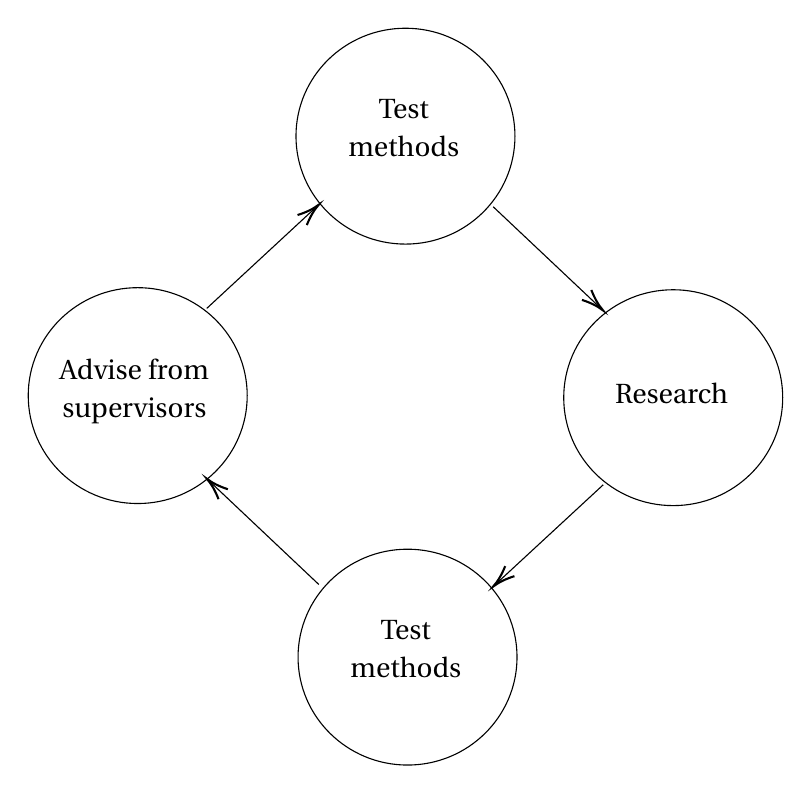
\begin{tikzpicture}[x=0.75pt,y=0.75pt,yscale=-1,xscale=1]
%uncomment if require: \path (0,427); %set diagram left start at 0, and has height of 427

%Shape: Ellipse [id:dp8381675984532289] 
\draw   (107.5,211) .. controls (107.5,182.28) and (131.12,159) .. (160.25,159) .. controls (189.38,159) and (213,182.28) .. (213,211) .. controls (213,239.72) and (189.38,263) .. (160.25,263) .. controls (131.12,263) and (107.5,239.72) .. (107.5,211) -- cycle ;
%Shape: Ellipse [id:dp8879090651544747] 
\draw   (236.5,86) .. controls (236.5,57.28) and (260.12,34) .. (289.25,34) .. controls (318.38,34) and (342,57.28) .. (342,86) .. controls (342,114.72) and (318.38,138) .. (289.25,138) .. controls (260.12,138) and (236.5,114.72) .. (236.5,86) -- cycle ;
%Shape: Ellipse [id:dp159469530573498] 
\draw   (365.5,212) .. controls (365.5,183.28) and (389.12,160) .. (418.25,160) .. controls (447.38,160) and (471,183.28) .. (471,212) .. controls (471,240.72) and (447.38,264) .. (418.25,264) .. controls (389.12,264) and (365.5,240.72) .. (365.5,212) -- cycle ;
%Shape: Ellipse [id:dp6243045365348194] 
\draw   (237.5,337) .. controls (237.5,308.28) and (261.12,285) .. (290.25,285) .. controls (319.38,285) and (343,308.28) .. (343,337) .. controls (343,365.72) and (319.38,389) .. (290.25,389) .. controls (261.12,389) and (237.5,365.72) .. (237.5,337) -- cycle ;
%Straight Lines [id:da3764417411513329] 
\draw    (193.5,169) -- (246.03,120.36) ;
\draw [shift={(247.5,119)}, rotate = 497.2] [color={rgb, 255:red, 0; green, 0; blue, 0 }  ][line width=0.75]    (10.93,-3.29) .. controls (6.95,-1.4) and (3.31,-0.3) .. (0,0) .. controls (3.31,0.3) and (6.95,1.4) .. (10.93,3.29)   ;
%Straight Lines [id:da08718773032378624] 
\draw    (384.5,254) -- (332.97,301.64) ;
\draw [shift={(331.5,303)}, rotate = 317.25] [color={rgb, 255:red, 0; green, 0; blue, 0 }  ][line width=0.75]    (10.93,-3.29) .. controls (6.95,-1.4) and (3.31,-0.3) .. (0,0) .. controls (3.31,0.3) and (6.95,1.4) .. (10.93,3.29)   ;
%Straight Lines [id:da9455012657988889] 
\draw    (331.5,120) -- (383.05,168.63) ;
\draw [shift={(384.5,170)}, rotate = 223.32999999999998] [color={rgb, 255:red, 0; green, 0; blue, 0 }  ][line width=0.75]    (10.93,-3.29) .. controls (6.95,-1.4) and (3.31,-0.3) .. (0,0) .. controls (3.31,0.3) and (6.95,1.4) .. (10.93,3.29)   ;
%Straight Lines [id:da04085276077852196] 
\draw    (247.5,302) -- (194.95,252.37) ;
\draw [shift={(193.5,251)}, rotate = 403.36] [color={rgb, 255:red, 0; green, 0; blue, 0 }  ][line width=0.75]    (10.93,-3.29) .. controls (6.95,-1.4) and (3.31,-0.3) .. (0,0) .. controls (3.31,0.3) and (6.95,1.4) .. (10.93,3.29)   ;

% Text Node
\draw (259.25,67) node [anchor=north west][inner sep=0.75pt]   [align=left] {\begin{minipage}[lt]{41.865356pt}\setlength\topsep{0pt}
    \begin{center}
    Test \\methods
        \end{center}

    \end{minipage}};
% Text Node
\draw (117.75,192) node [anchor=north west][inner sep=0.75pt]   [align=left] {\begin{minipage}[lt]{59.42064400000001pt}\setlength\topsep{0pt}
    \begin{center}
    Advise from \\supervisors
        \end{center}

    \end{minipage}};
% Text Node
\draw (385.25,203.5) node [anchor=north west][inner sep=0.75pt]   [align=left] {\begin{minipage}[lt]{46.398644000000004pt}\setlength\topsep{0pt}
    \begin{center}
    Research
        \end{center}

    \end{minipage}};
% Text Node
\draw (260.25,318) node [anchor=north west][inner sep=0.75pt]   [align=left] {\begin{minipage}[lt]{41.865356pt}\setlength\topsep{0pt}
    \begin{center}
    Test \\methods
        \end{center}

    \end{minipage}};


\end{tikzpicture}

\captionof{figure}{Illsutration of workflow}
\label{fig:workflow}
\end{tabular}

\subsection{Structure of report}
TODO

\subsection{Definition of important terms} \label{sec:definitions}
\subsubsection{Cyber-Physical Systems(CPS)}\label{sec:cps}
Cyber-Physical Systems(CPS) can be defined as "engineered systems that integrate information technologies, real‐time control subsystems, physical components, and human operators to influence physical processes by means of cooperative and (semi)automated control functions."~\cite{guzman_wied_kozine_lundteigen_2019}
CPS is a broad term, and examples can be everything automated control systems at offshore platforms to the computer system in an electric car. As more and more of the CPSs are connected to the internet, cyber threats becomes a bigger challenge. 

\subsubsection{Open-Source Intelligence(OSINT)}\label{sec:osint}
Open-Source Intelligence(OSINT) is defined by the American Office of The Director of National Intelligence in their Intelligence Community Directive as: "[Intelligence] produced from publicly available information that is collected, exploited, and disseminated in a timely manner to an appropriate audience for the purpose of addressing a specific intelligence requirement."\cite{directive_301} This directive also defines Open Source Information as "Publicly available information that anyone can lawfully obtain by request, purchase, or observation.". Open-Source Intelligence (OSINT) is therefore gathering of intelligence that is lawfully available to the public. 


\section{Theory}

\subsection{IPv4}
To navigate the internet, the IP protocol is used. This is mainly split into the popular IPv4 and the new IPv6. IPv4 addresses are 32 bit, meaning they can range from 0.0.0.0 to 255.255.255.255. 

\subsubsection{IPv6}
The solution to the exhaustion of IPv4 address space is IPv6. This protocol has $2^{128}$ unique addresses, so it will be able to cover the forseable future. The global conversion from IPv4 to IPv6 is slow, however.While Shodan does support IPv6, most corporations in the maritime and offshore industries are big enough to have, and use, IPv4 addresses. 


\subsection{IP range}
 The IPv4 addresses are sold to organisations, for them to distribute further. For example, an Internet Service Provider (ISP) like Telenor will give IPv4 addresses to the customers while they use their subscribed internet connections. This distribution of IPv4 addresses to organisations is illustrated in \cref{fig:ipv4_map}.

\begin{figure}
    \centering
    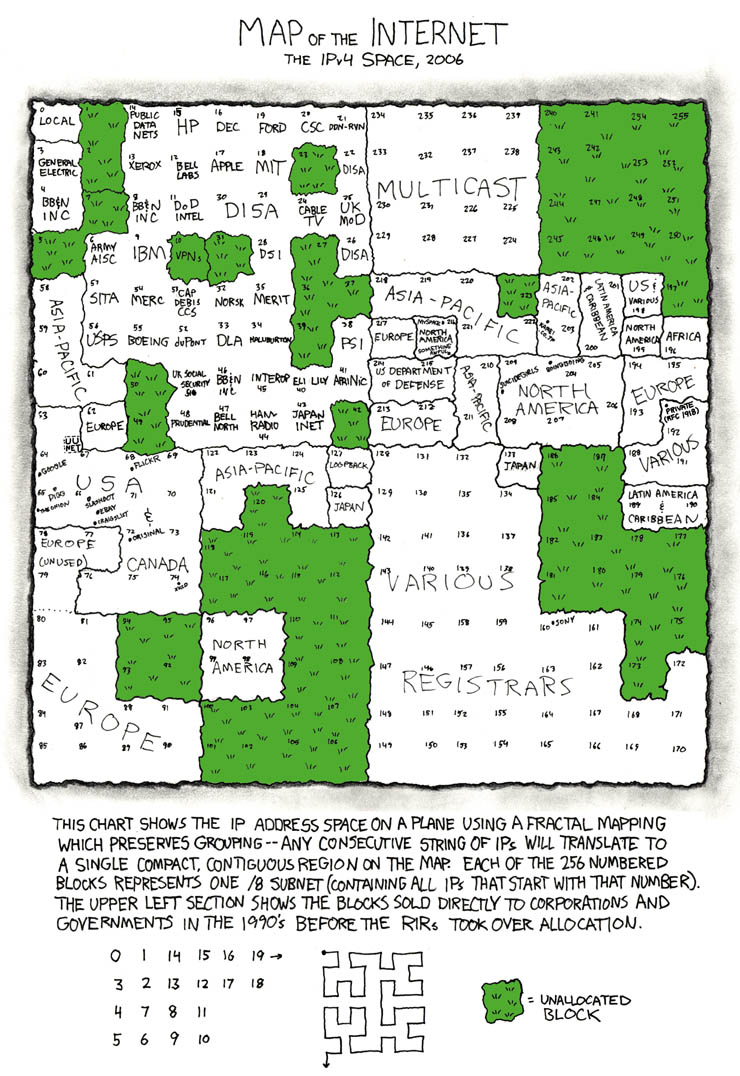
\includegraphics[scale=4]{Figurer/map_of_the_internet.jpg}
    \caption{A map of the IPv4 space, from the XKCD webcomic. \cite{xkcd} }
    \label{fig:ipv4_map}
\end{figure}

\subsubsection{IPv4 exhaustion and NAT}
IPv4 addresses were distributed by the Internet Assigned Numbers Authority (IANA). 11 January, 2011, IANA allocated its last block.\cite{exhasuted_IPV4} Since then, the regional bodies responsible for allocationg IPv4 addresses, Regional Internet Registries (RIR), have also exhausted their IPv4 addresses, the last one in 2019.\cite{exhausted_RIPENNC} Due to this problem, multiple methods are used to get the most out of the IPv4 address space. Arguably, the most popular of these methods are Network Address Translation (NAT).

NAT lets you connect multiple devices to the same IPv4. This is done by using a routing device with a shared IPv4 address to receive packages for multiple different devices, and then redirect the packages to the correct receiver. This makes it so that the devices behind the NAT can reach the internet, while communication from the internet can not reach the devices unless the devices start the communication. This connection is illustrated in \cref{fig:NAT} 

\tikzset{every picture/.style={line width=0.75pt}} %set default line width to 0.75pt        
\begin{tabular}{p{10cm}}
   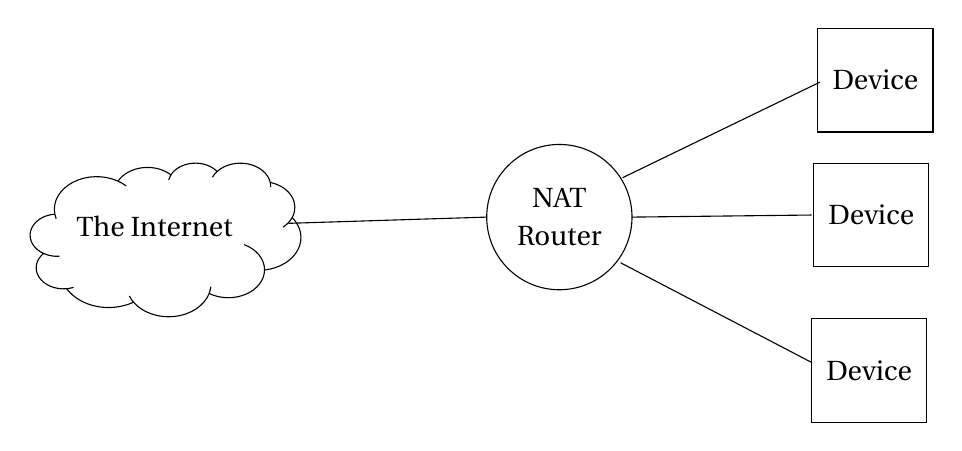
\begin{tikzpicture}[x=0.75pt,y=0.75pt,yscale=-1,xscale=1]
     %uncomment if require: \path (0,300); %set diagram left start at 0, and has height of 300

%Shape: Rectangle [id:dp7550808737565868] 
\draw   (417.5,74) -- (473,74) -- (473,124) -- (417.5,124) -- cycle ;

%Shape: Ellipse [id:dp5744265006375734] 
\draw   (258,165) .. controls (258,145.67) and (273.67,130) .. (293,130) .. controls (312.33,130) and (328,145.67) .. (328,165) .. controls (328,184.33) and (312.33,200) .. (293,200) .. controls (273.67,200) and (258,184.33) .. (258,165) -- cycle ;

%Straight Lines [id:da011152119100300673] 
\draw    (418.5,100) -- (323.5,146) ;
%Shape: Rectangle [id:dp019726233695570805] 
\draw   (414.5,214) -- (470,214) -- (470,264) -- (414.5,264) -- cycle ;

%Shape: Rectangle [id:dp2854982925574172] 
\draw   (415.5,139) -- (471,139) -- (471,189) -- (415.5,189) -- cycle ;

%Straight Lines [id:da042657718924057675] 
\draw    (414.5,164) -- (328,165) ;
%Straight Lines [id:da8590380439733557] 
\draw    (414.5,235) -- (322.5,187) ;
%Shape: Cloud [id:dp5209862047408297] 
\draw   (49.88,163.36) .. controls (48.82,157.4) and (52.27,151.49) .. (58.76,148.15) .. controls (65.25,144.81) and (73.64,144.62) .. (80.36,147.67) .. controls (82.74,144.2) and (87.1,141.8) .. (92.13,141.21) .. controls (97.15,140.61) and (102.24,141.88) .. (105.86,144.64) .. controls (107.89,141.49) and (111.87,139.38) .. (116.4,139.05) .. controls (120.93,138.71) and (125.35,140.21) .. (128.11,143.01) .. controls (131.78,139.67) and (137.61,138.27) .. (143.09,139.4) .. controls (148.57,140.54) and (152.7,144) .. (153.71,148.31) .. controls (158.2,149.25) and (161.95,151.66) .. (163.97,154.91) .. controls (166,158.15) and (166.1,161.92) .. (164.27,165.23) .. controls (168.7,169.68) and (169.73,175.61) .. (166.99,180.8) .. controls (164.25,186) and (158.14,189.68) .. (150.95,190.48) .. controls (150.9,195.35) and (147.44,199.83) .. (141.9,202.17) .. controls (136.37,204.52) and (129.62,204.38) .. (124.26,201.79) .. controls (121.98,207.63) and (115.55,211.93) .. (107.76,212.83) .. controls (99.97,213.73) and (92.21,211.06) .. (87.83,205.99) .. controls (82.46,208.49) and (76.02,209.21) .. (69.96,207.99) .. controls (63.9,206.77) and (58.74,203.7) .. (55.62,199.49) .. controls (50.14,199.99) and (44.84,197.79) .. (42.35,194) .. controls (39.86,190.2) and (40.71,185.61) .. (44.49,182.5) .. controls (39.59,180.28) and (37.1,175.87) .. (38.3,171.56) .. controls (39.5,167.26) and (44.13,164.05) .. (49.76,163.59) ; \draw   (44.49,182.5) .. controls (46.8,183.55) and (49.46,184.03) .. (52.13,183.87)(55.62,199.49) .. controls (56.77,199.39) and (57.89,199.17) .. (58.97,198.84)(87.83,205.99) .. controls (87.02,205.06) and (86.34,204.06) .. (85.81,203.01)(124.26,201.79) .. controls (124.67,200.73) and (124.95,199.63) .. (125.06,198.52)(150.95,190.48) .. controls (151.01,185.28) and (147.19,180.53) .. (141.14,178.26)(164.27,165.23) .. controls (163.29,167) and (161.79,168.57) .. (159.9,169.81)(153.71,148.31) .. controls (153.88,149.02) and (153.95,149.75) .. (153.94,150.47)(128.11,143.01) .. controls (127.2,143.84) and (126.44,144.77) .. (125.87,145.77)(105.86,144.64) .. controls (105.37,145.39) and (105.01,146.19) .. (104.77,147.02)(80.36,147.67) .. controls (81.78,148.31) and (83.1,149.09) .. (84.28,149.97)(49.88,163.36) .. controls (50.02,164.19) and (50.25,165) .. (50.56,165.79) ;

%Straight Lines [id:da9624009852798121] 
\draw    (162.5,168) -- (258,165) ;

% Text Node
\draw (293,165) node   [align=left] {\begin{minipage}[lt]{33.354pt}\setlength\topsep{0pt}
\begin{center}
NAT\\Router
\end{center}

\end{minipage}};
% Text Node
\draw (445.25,99) node   [align=left] {Device};
% Text Node
\draw (442.25,239) node   [align=left] {Device};
% Text Node
\draw (443.25,164) node   [align=left] {Device};
% Text Node
\draw (59,163) node [anchor=north west][inner sep=0.75pt]   [align=left] {The Internet};

   \end{tikzpicture}
   \captionof{figure}{Illustration of a NAT router}
   \label{fig:NAT}
\end{tabular}


\subsubsection{CIDR}
 Classless Inter-Domain Routing(CIDR) is the modern way to split the IPv4 address space into blocks, so that they can be distributed. A CIDR block can look like this: "93.192.0.0/10". This block has two parts, the prefix "93.192.0.0" and the suffix "/10". The prefix indicates the size of the CIDR block. The prefix indicates where in the IPv4 space the CIDR block is located. To understand this, it is useful to look at an IP address in binary instead of decimal. For example, the IPv4 address "93.220.107.30" becomes "01011101.11011100.01101011.00011110". The suffix decides how many bits are fixed. In the CIDR block "93.220.107.30/10", the 10 first bits of the prefix "93.220.107.30"  are "01011101.11xxxxxx.xxxxxxxx.xxxxxxxx". This number span the binary range \\ \{01011101.11111111.11111111.11111111 - 01011101.11000000.00000000.00000000 \}, or the decimal range  \{ 93.192.0.1 - 93.255.255.254 \}. Remark that not the full prefix is needed; "93.220.107.30/10" and "93.220.107.31/10" are the same CIDR  block. Because of this, it is normal to set the changing bits of the prefix to 0, as in: "93.192.0.0/10". 
Since the sizes of CIDR blocks vary, they can be nested. For example, "93.192.0.0/11" is a part of "93.192.0.0/10".


\subsection{Shodan}\label{sec:shodan}
Shodan is a search engine like Google. Instead of searching for web pages, however, it will gather publicly-available information about all devices directly connected to the internet.~\cite{shodan} This makes Shodan ideal for mapping all CPSs that are connected to the internet.

\subsubsection{Shodan account}
It is possible to make up to 5 queries using Shodan without registering an account. 
With a free account, it is possible to perform more queries, access the Shodan API, and get limited access to search filters. However, without a paid account, the search engine has limitations.
Using the API, a free user can access up to 100 results from searches. 
For paid users, there are three payment plans: Freelancer, Small Business and Corporate. A Freelancer user gets access to up to 1 million results per month and access to most search filters. 
Users paying for the higher tiers can get from 20 million to an unlimited number of results, all search filters and multiple extra benefits. 
The Freelancer payment plan will be sufficient for the scope of this project.

\subsubsection{Crawlers and banners}
Shodan has bots called "crawlers" to find information about devices connected to the internet, such as IP address, port number, country, service running, version, protocols used, and more. 
All these properties are saved in Shodan "banners" . The creator of Shodan, John Matherly has described banners as "A banner is simply metadata about a service.". \cite{banner} 
Therefore, when a user starts a search using the Shodan search engine, it will not return live results, but rather the banners already saved in the Shodan database. Shodan guarantees that returned banners have been collected in the last 30 days.\cite{matherly_guide_to_shodan}
Some of the Shodan banner properties are always on banners, while others are situational. For example will SSL properties only occur on banners of ports that use SSL encryption. A complete list of both required and situational Shodan banner properties can be found in \cref{app:banner_properties}.
Normally, the banners are in the JSON format. An example of a banner can be found in \cref{app:marlink_banner}.
Matherly\cite{matherly_guide_to_shodan} describes the basic algorithm for Shodan crawlers as:
\begin{enumerate}
\setlength\itemsep{0em}
	\item Generate a random IPv4 address. 
	\item Generate a random port to test from the list of ports that Shodan understands.
	\item Check the random IPv4 address on the random port and grab a banner.
	\item Goto 1
\end{enumerate}
The list of ports mentioned can be found by using the API web call in \cref{lst:api_ports}.

\subsubsection{Search filters} \label{sec:filters}
To limit the results returned from a Shodan query, filters are applied. Filters are on the format:
\begin{lstlisting}
filter_property: value
\end{lstlisting}
When using a filter, Shodan queries will return banners where the properties specified in the filter contain the specified value. In most cases, filter properties correspond with banners. However, some filter properties are not banner properties. For example the "geo" filter property can define an area. The Shodan query will then return all banners where the "location.latitude" and "location.longitude" properties are within this area. 

A comprehensive list of the Shodan filters can be found in \cref{app:shodan_filters}, . The queries used in this project will be explained in more detail. 

\subsection{Previous research}
Since Shodan was launched in 2009, a lot of research has been done in order to finding ICS using Shodan. The Shodan website even has its own article on the subject.\cite{shodan_ics} There also exist other lists of Shodan queries that will find ICS systems. For example, the website SCADA Strangelove has compiled multiple such lists, focusing on both Supervisory Control And Data Acquisition (SCADA) and ICS devices.\cite{scadasl_cheatsheet} \cite{scadasl_shodan}

On the other hand, research exist on ICS defense against Shodan scans. For example, \textit{Evaluation of the ability of the Shodan search engine to identify Internet-facing industrial control devices} by Bodenheim, Butts, Dunlap and Mullins, \cite{bodenheim_butts_dunlap_mullins_2014} demonstrates how obfuscation can be used to mask ICS devices from Shodan searches. Furthermore, the article implemented this on several honeypots. A honeypot is a computer that is configured to look like another device, in this case an ICS. Then the honeypot will log all traffic. Bodenheim, Butts, Dunlap and Mullins had an independent researcher try to find the devices using Shodan, showing how the devices were harder to find when obfuscated.

\newpage


\section{Selective identification of IP devices} \label{sec:method}
As described in \cref{sec:research_approach}, methods are suggested to find devices as per the project goal. 
This chapter describes these suggested methods, based on the theory from \cref{sec:theory}.

Several methods to filter devices based on what industries they belong to, are suggested in \cref{sec:identify_industry}. These methods are not exclusive, and multiple methods may for example be combined to double-check the validity of the results. In \cref{sec:identify_cps}, additional methods are suggested on how to identify if devices are part of a Cyber-Physical System.

\subsection{Identifying devices from specific industries} \label{sec:identify_industry}
\subsubsection{Banner similarities} \label{sec:banner_method}
When connecting a device to the internet, it needs to be configured. The configurer needs competence and time to do this properly. To make such devices more accessible and efficient, ready-made solutions are most often used. Due to this, the devices mainly have the same default configuration, and therefore identical banners. This can be used to identify devices by using the following method.
\begin{enumerate}
    \item Choose a device type that fulfills the constraints and may be connected to the internet.
    \item Find the IP address of one instance of such a device, and find its Shodan entry.
    \item Get its banner.
    \item Use unique information from the banner to find all devices with similar banners.
\end{enumerate}
The most difficult of these steps is to find the IP address. The easiest way to do this is to be in possession of, and have ownership to, the device, and find its IP address through administrative privileges. 
If this is not an option, the device could be found by guessing what information is in its banner, for example the device name or open ports.
Unfortunately, this project does not have access to devices that fit the goals described in \cref{sec:objectives}.

\subsubsection{Internet Service Provider and IP ranges} \label{sec:isp_method}
Internet Service Providers(ISP) are the organizations that connect people and companies to the internet. ISPs charge money to deliver internet connectivity, and most people have a subscription. Telenor is for example a Norwegian ISP. While a lot of ISPs are generalized and deliver the internet to both private and organizational customers, others can be more specialized. 

Regional Internet Registries (RIR) sell IP addresses to organizations, for them to distribute further. For example, an Internet Service Provider(ISP) will buy a CIDR range, then give IPv4 addresses to customers while they use their subscribed internet connections. An overview of the distribution of IPv4 addresses to organizations is illustrated in \cref{fig:ipv4_map}. Shodan can use the filter "isp" to search for ISPs, "org" to search for organizations, and "net" to search for devices in a CIDR range. 

\begin{figure} [H]
    \centering
    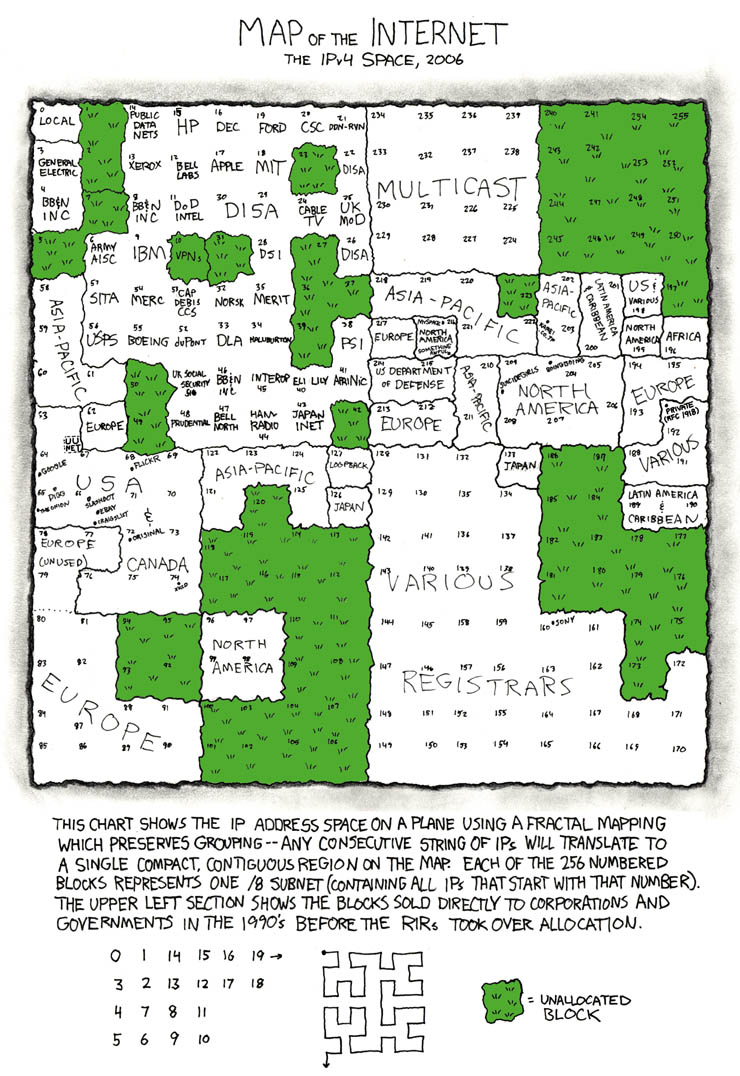
\includegraphics[scale=4]{Figurer/map_of_the_internet.jpg}
    \caption{A map of the IPv4 space, from the XKCD webcomic. \cite{xkcd} }
    \label{fig:ipv4_map}
\end{figure}

While it often is an uncomplicated procedure to find the name of an organization or ISP, a tool is needed to find CIDR ranges. One or more CIDR ranges owned by an organization and with a single defined routing policy, is called an Autonomous System(AS). A typical example of an organization that owns an AS, is an Internet Service Provider(ISP). \cite{AS_def} 
The ASs are registered with unique identification numbers. Online tools, like \href{https://hackertarget.com/as-ip-lookup/}{\textbf{Hackertarget AS-IP lookup}} \cite{asip_lookup}, make it possible to find the parent AS of an IP address. Then the rest of the IP addresses belonging to the same AS can be found.


\subsubsection{Reverse IP geolocation} \label{sec:geo_method}
When Regional Internet Registries (RIR) give IP addresses to organizations, they also register contact information on the IP addresses. Part of this information is a location, specifying a country and a city. Some data providers claim that the country accuracy is between 95\% and 99\%, while the city accuracy is between 50\% and 75\%.\cite{geolocation_acc} With accuracy that poor, it is not possible to use IP geolocation to decisively determine the location an IP address. The information returned by one of the RIRs can be seen in \cref{fig:RIPE_NCC}.
Shodan has a filter for the location. This filter can also query by latitude and longitude. However, Shodan does not disclose how they gather this information. 
Because of these uncertainties, IP geolocation can not be conclusive for identifying devices. However, by reversing the technique, it would be possible to narrow down the selection of IP addresses by first defining a geographical area. Shodan can use the filter "geo:latitude,longitude,radius" to filter addresses by location.  

\begin{figure} [H]
    \centering
    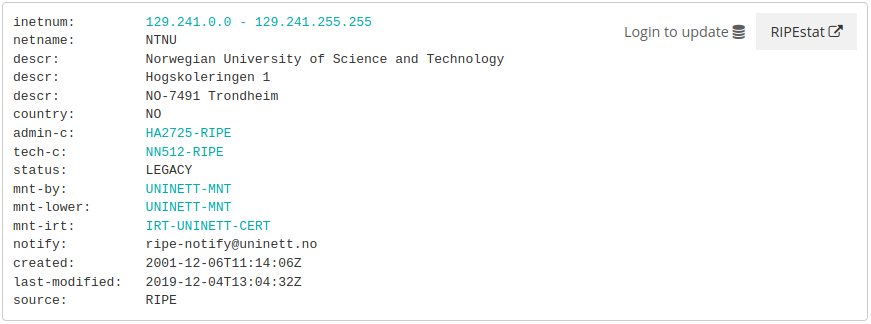
\includegraphics[scale=0.5]{Figurer/ripe.png}
    \caption{The IP address lookup of RIPE NCC \cite{ripe_whois}}
    \label{fig:RIPE_NCC}
\end{figure}

\subsubsection{Latency and traceroute} \label{sec:latency_method}
The simplest form of reaching another device on the internet is called a "ping". This sends a echo request to an IP address, to make it send a response back. It is mainly used to check if a device is reachable. To prevent a bug where packets travel in an infinite loop instead of reaching the recipient, packets have a Time To Live (TTL) counter. The packet increments a variable every time a it travels through a switch or router. When this variable reaches the TTL counter , the packet is stopped, and a message is returned to the sender, informing it of the loss.
The "traceroute" command takes advantage of the fact that the Time To Live counter can be set by the sender. It will start the TTL counter at 1 and will send a message towards a predefined target IP address. This message will then travel 1 step towards its target before it is returned. Then traceroute increments this counter and repeats the send. This way, all routers that the packet travels through on its way, will be indexed. In addition, traceroute will time how long the packet uses before it is returned, called "Round Trip Time"(RTT).
The Round Trip Time can give an idea of how the signal travels. Faster RTT can the result of shorter distance or better infrastructure. Vice versa, slow RTT may indicate longer distance or worse infrastructure.
The traceroute is visualized in \cref{fig:latency}. Here the signal will travel fast from Source to both Router 1 and Router 2. There will then be a jump in latency when the signal crosses the Atlantic ocean on its way to router 3. The longest delay will be where the signal travels to the Destination from Router 3 via a satellite.

\begin{figure} [H]
    \centering
    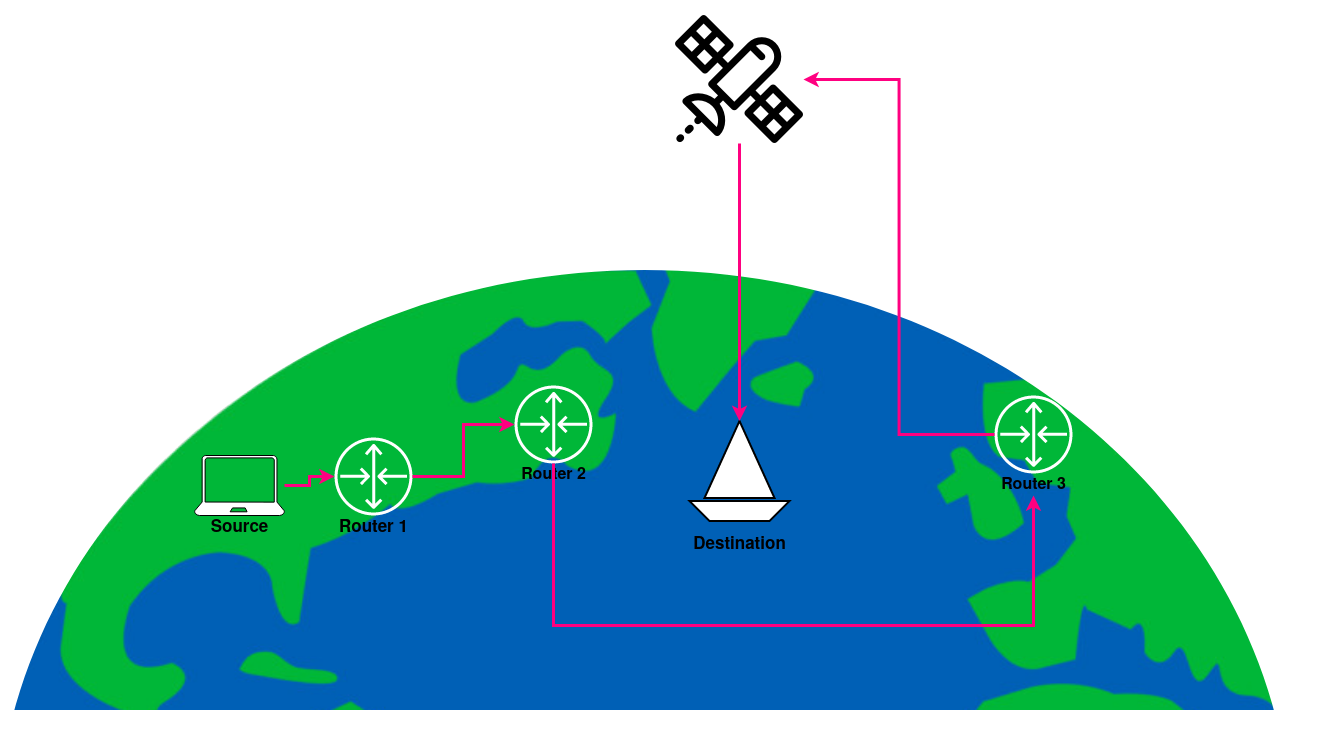
\includegraphics[scale=0.3]{Figurer/latency.png}
    \caption{Visualization of internet latency. Map from \href{http://getdrawings.com/earth-cartoon-drawing}{http://getdrawings.com/earth-cartoon-drawing}}
    \label{fig:latency}
\end{figure}

\subsection{Identifying devices from Cyber-Physical Systems} \label{sec:identify_cps}
As mentioned in \cref{sec:cps}, Cyber-Physical Systems(CPS) are systems containing anything from real-time controllers to human operators. Not all CPS have components that are connected to the internet. When a CPS is connected to the internet, only some of its components are actually connected. In the offshore industry, CPSs are typically Industrial Control Systems(ICS). In the maritime industry, CPSs are typically navigation systems. As these industries often overlap, their CPS use-cases often overlap as well. Methods for identifying two subsections of CPS, ICS and navigation systems will be proposed below.
These methods can be used separately, but in this project they are intended for use on a subset of devices that are filtered from the methods suggested in \cref{sec:identify_industry}.

\subsubsection{Industrial Control Systems}
Industrial Control Systems(ICS) are in most cases easy to identify. A lot of previous research already exists on how to use Shodan to identify ICS. For example: \textit{Exploring Shodan From the Perspective of Industrial Control Systems}\cite{bodenheim_butts_dunlap_mullins_2014} and \textit{Evaluation of the ability of the Shodan search engine to identify Internet-facing industrial control devices} \cite{ICS_shodan_article}.  In addition, Shodan has a list of popular ICS and search terms used to find the systems.\cite{shodan_ics} The different ICSs use standard ports for communication through the internet, and Shodan can use the "port" filter to find them. ICSs often have similar banners, and the same method as in \cref{sec:banner_method} would work on ICSs.

\subsubsection{Navigation systems}
In the maritime industry, Electronic Chart Display and Information System(ECDIS) is often used for navigating ships. While a lot of them have downloaded maps, many also use online maps, and therefore has a connection to the internet. For identifying these systems, the methods proposed in \cref{sec:banner_method} and \cref{sec:isp_method} would be the most effective.

\newpage

\section{Implementation and results} \label{sec:results}
This project implemented the different approaches to selective identification of IP devices proposed in \cref{sec:method}. These implementations, along with a discussion of the results, will be described here. 


\subsection{Banner similarities} \label{sec:banner_results}
Following the approach proposed in \cref{sec:banner_method}, the first step is to choose a type of device that could fit the constraints of this project. Two methods was used to find a such a device. The first one was to find other research into the same area, and look at their results. Google Scholar\cite{google_scholar} and Engineering Village\cite{engineering_village} was used in search for articles on the subject, while DuckDuckGo\cite{ddg} was used to search for other sources. A PowerPoint presentation from the Hack In The Box Security Conference 2018 was found, named \textit{Hacking yachts remotely}. This presentation illustrates different methods to hack Yachts. Here the search query "Maritime Stabilized Antenna System" was used to find internet connected antennas of the model "Cobham Seatel Satcom". 
"Marine Stabilized Antenna System" would then be an identifying part of the banner of this device. The 22 results found when using Shodan to search for this can be found in \cref{fig:banner_parsing}. Note that all devices run on the same port: 161, which is used for the Simple Network Management Protocol (SNMP). This will be looked further into in \cref{sec:combo}.

\begin{figure} [H]
    \centering
    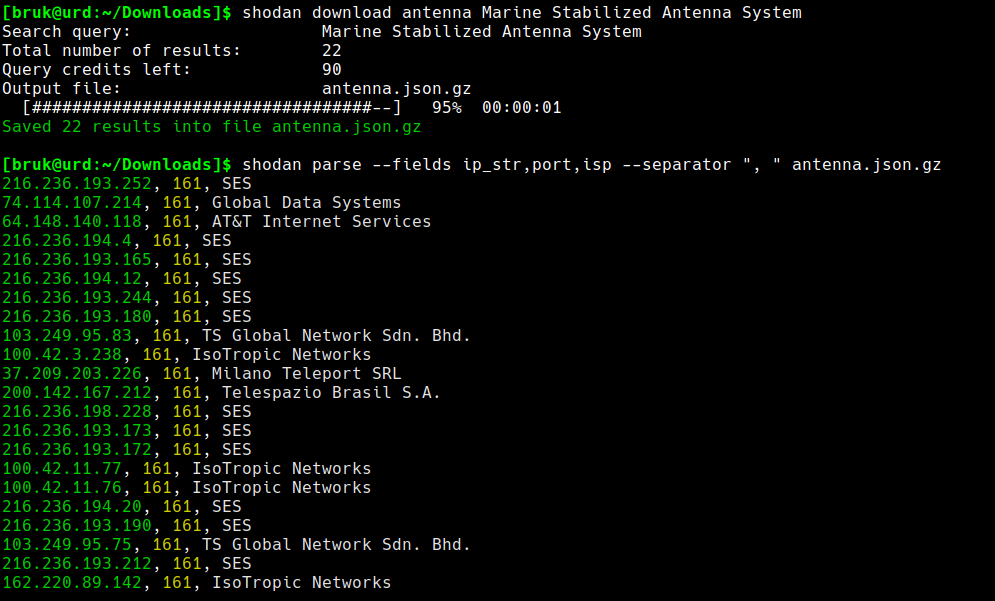
\includegraphics[scale=0.4]{Figurer/banner_parsing.png}
    \caption{Using the Shodan CLI to download and parse results. Results are listed with IP addresses, open ports and ISP.}
    \label{fig:banner_parsing}
\end{figure}

In the millions of devices connected to the internet, 22 devices is not really very many. However, this is the most accurate device identification this project was able to do. While the other approaches are also able to identify devices, it is not certain that those are a part of the offshore or maritime industries. The Cobham Seatel Satcom antenna is definitely a part of the navigation system of a ship, which is a maritime Cyber-Physical System. This one result was also one not found by this project, but by another project. More specifically, it was found by someone who has more insight into the industry, showing that device identification by banner specification is easier with experience from area of work within the constraints or access to relevant devices.

If this experience or access is not available, like in this project, a couple of methods can be used to search for identifying device banners. 
Some technologies are intended for specialized use. For example the NMEA communication standard for marine sensors and display units. \cite{NMEA} This will of course be mostly used in the marine industry. A Shodan search for "NMEA" shows that 88 IP addresses have the word NMEA in their description. While some of those devices probably use NMEA to communicate, some might just have the letters "NMEA" in their banner as a coincidence. This can be the case with short search terms. The port 10110 is intended for NMEA 0183 Navigational Data. \cite{www_ports} A search for this port with Shodan returns 6 results, which is quite low. 
It is possible to find devices that are used within a industry, in this case either maritime or offshore. These devices need to be specific for the industry, as findings will not be decisive if the devices can be found in used not within the constraints. To find the right devices, one approach can be to find producers or resellers of equipment for a specific industry. A list of manufacturers of NMEA equipment can be found at \cite{NMEA}. It is logical that some of these manufacturers would also make equipment for the marine industry that is not NMEA. 
Some time of this project was spent in search of identifiable banners, but nothing as clear as the Maritime Stabilized Antenna System was found in the search. 
%\todo[inline]{Finish this section by adding results from table or something.}


\subsection{ISP}
For identifying devices by looking at Internet Service Providers (ISP), Tampnet will be used as an example. On their webpage, the following can be found: "By providing a fast subsea fibre optic network and 4G LTE coverage, Tampnet enables digitalization of offshore operations within oil \& gas, maritime and wind energy." \cite{tampnet} Tampnet is an ISP that provides internet connections to the maritime, offshore and wind energy industries. 

\begin{figure} [H]
    \centering
    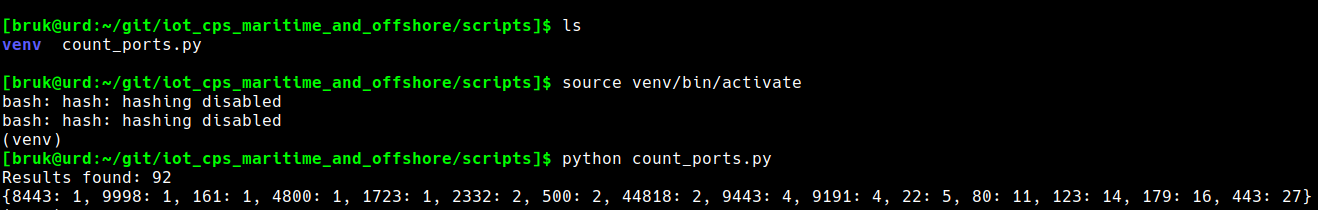
\includegraphics[scale=0.35]{Figurer/python_ports.png}
    \caption{The output from a python script that is counting the different number of ports open by the devices returned from the Shodan query "isp:tampnet". The script is "count\_ports.py" at \cite{scripts}}
    \label{fig:tampnet_ports}
\end{figure}

This query returns 92 different IP addresses belonging to Tampnet. This approach is not definitive, however, since there is no way of knowing if these devices are a part of a cyber-physical system in the offshore industry. Even so, these 92 devices has a higher chance of being within the constraints than other random devices on the internet. This method will thus act more as a filter for finding potential hits. 

The Hackertarget AS lookup tool \cite{asip_lookup} is used to find that Tampnet own the CIDR range "185.96.40.0/22", which is 1024 available IP addresses. \cite{CIDR_table} Therefore, Tampnet probably has more than 92 active IP addresses as part of their ISP. Shodan can not find the rest of the IP addresses of Tampnet since they can not be reached from the public internet. One reason for this could be that Tampnet employs a firewall to filter what IP addresses are able to find their address. This is called whitelisting, where only a selected number of devices can communicate through the router with a firewall, as illustrated in \cref{fig:firewall}.


\tikzset{every picture/.style={line width=0.75pt}} %set default line width to 0.75pt
\begin{tabular}{p{10cm}}
    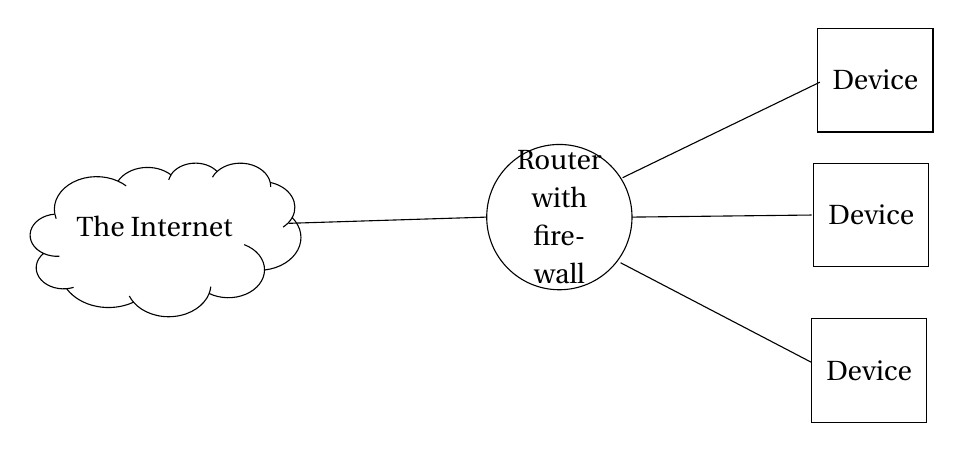
\begin{tikzpicture}[x=0.75pt,y=0.75pt,yscale=-1,xscale=1]
        %uncomment if require: \path (0,300); %set diagram left start at 0, and has height of 300

        %Shape: Rectangle [id:dp7550808737565868]
        \draw   (417.5,74) -- (473,74) -- (473,124) -- (417.5,124) -- cycle ;

        %Shape: Ellipse [id:dp5744265006375734]
        \draw   (258,165) .. controls (258,145.67) and (273.67,130) .. (293,130) .. controls (312.33,130) and (328,145.67) .. (328,165) .. controls (328,184.33) and (312.33,200) .. (293,200) .. controls (273.67,200) and (258,184.33) .. (258,165) -- cycle ;

        %Straight Lines [id:da011152119100300673]
        \draw    (418.5,100) -- (323.5,146) ;
        %Shape: Rectangle [id:dp019726233695570805]
        \draw   (414.5,214) -- (470,214) -- (470,264) -- (414.5,264) -- cycle ;

        %Shape: Rectangle [id:dp2854982925574172]
        \draw   (415.5,139) -- (471,139) -- (471,189) -- (415.5,189) -- cycle ;

        %Straight Lines [id:da042657718924057675]
        \draw    (414.5,164) -- (328,165) ;
        %Straight Lines [id:da8590380439733557]
        \draw    (414.5,235) -- (322.5,187) ;
        %Shape: Cloud [id:dp5209862047408297]
        \draw   (49.88,163.36) .. controls (48.82,157.4) and (52.27,151.49) .. (58.76,148.15) .. controls (65.25,144.81) and (73.64,144.62) .. (80.36,147.67) .. controls (82.74,144.2) and (87.1,141.8) .. (92.13,141.21) .. controls (97.15,140.61) and (102.24,141.88) .. (105.86,144.64) .. controls (107.89,141.49) and (111.87,139.38) .. (116.4,139.05) .. controls (120.93,138.71) and (125.35,140.21) .. (128.11,143.01) .. controls (131.78,139.67) and (137.61,138.27) .. (143.09,139.4) .. controls (148.57,140.54) and (152.7,144) .. (153.71,148.31) .. controls (158.2,149.25) and (161.95,151.66) .. (163.97,154.91) .. controls (166,158.15) and (166.1,161.92) .. (164.27,165.23) .. controls (168.7,169.68) and (169.73,175.61) .. (166.99,180.8) .. controls (164.25,186) and (158.14,189.68) .. (150.95,190.48) .. controls (150.9,195.35) and (147.44,199.83) .. (141.9,202.17) .. controls (136.37,204.52) and (129.62,204.38) .. (124.26,201.79) .. controls (121.98,207.63) and (115.55,211.93) .. (107.76,212.83) .. controls (99.97,213.73) and (92.21,211.06) .. (87.83,205.99) .. controls (82.46,208.49) and (76.02,209.21) .. (69.96,207.99) .. controls (63.9,206.77) and (58.74,203.7) .. (55.62,199.49) .. controls (50.14,199.99) and (44.84,197.79) .. (42.35,194) .. controls (39.86,190.2) and (40.71,185.61) .. (44.49,182.5) .. controls (39.59,180.28) and (37.1,175.87) .. (38.3,171.56) .. controls (39.5,167.26) and (44.13,164.05) .. (49.76,163.59) ; \draw   (44.49,182.5) .. controls (46.8,183.55) and (49.46,184.03) .. (52.13,183.87)(55.62,199.49) .. controls (56.77,199.39) and (57.89,199.17) .. (58.97,198.84)(87.83,205.99) .. controls (87.02,205.06) and (86.34,204.06) .. (85.81,203.01)(124.26,201.79) .. controls (124.67,200.73) and (124.95,199.63) .. (125.06,198.52)(150.95,190.48) .. controls (151.01,185.28) and (147.19,180.53) .. (141.14,178.26)(164.27,165.23) .. controls (163.29,167) and (161.79,168.57) .. (159.9,169.81)(153.71,148.31) .. controls (153.88,149.02) and (153.95,149.75) .. (153.94,150.47)(128.11,143.01) .. controls (127.2,143.84) and (126.44,144.77) .. (125.87,145.77)(105.86,144.64) .. controls (105.37,145.39) and (105.01,146.19) .. (104.77,147.02)(80.36,147.67) .. controls (81.78,148.31) and (83.1,149.09) .. (84.28,149.97)(49.88,163.36) .. controls (50.02,164.19) and (50.25,165) .. (50.56,165.79) ;

        %Straight Lines [id:da9624009852798121]
        \draw    (162.5,168) -- (258,165) ;

        % Text Node
        \draw (293,165) node   [align=left] {\begin{minipage}[lt]{33.354pt}\setlength\topsep{0pt}
            \begin{center}
                Router\\ with \ firewall
            \end{center}

        \end{minipage}};
        % Text Node
        \draw (445.25,99) node   [align=left] {Device};
        % Text Node
        \draw (442.25,239) node   [align=left] {Device};
        % Text Node
        \draw (443.25,164) node   [align=left] {Device};
        % Text Node
        \draw (59,163) node [anchor=north west][inner sep=0.75pt]   [align=left] {The Internet};

    \end{tikzpicture}
    \captionof{figure}{Illustration of firewall functionality}
    \label{fig:firewall}
\end{tabular}

While Tampnet is an ISP in the Offshore industry, Marlink is a maritime satellite provider. The Shodan CLI query "shodan count isp:marlink" tell us that 5895 different IP addresses are online. While this is a lot more hits than for the Tampnet search, the same uncertainty remains: More tests have to be done to find what devices these really are. 

\subsection{Reverse Geolocation}
With many major seaports, like Rotterdam, Antwerp and Hamburg, the North Sea has a lot of marine traffic. The sea also has a lot of offshore oil and gas fields; Ekofisk, Sleipner, Forties and Valhall, to mention a few.\cite{oil_field_lists} With this much activity within both constraints, the marine and offshore industries, a lot of things in the area have to be connected to the internet. To test if the IP geolocation services of Shodan could detect devices connected to the internet, a large area of the North sea was chosen: a circle with 270 km around 56\degree24\textquotesingle00.0N 3\degree00\textquotesingle36.0E, as seen in \cref{fig:geolocation}. To use Shodan to find devices within this area, the command \cref{lst:geolocation_sea} was used. As seen in the output from the command, no devices was found within the area. The command syntax is "shodan count geo:LONGITUDE,LATITUDE,RADIUS"

\begin{figure} [H]
    \centering
    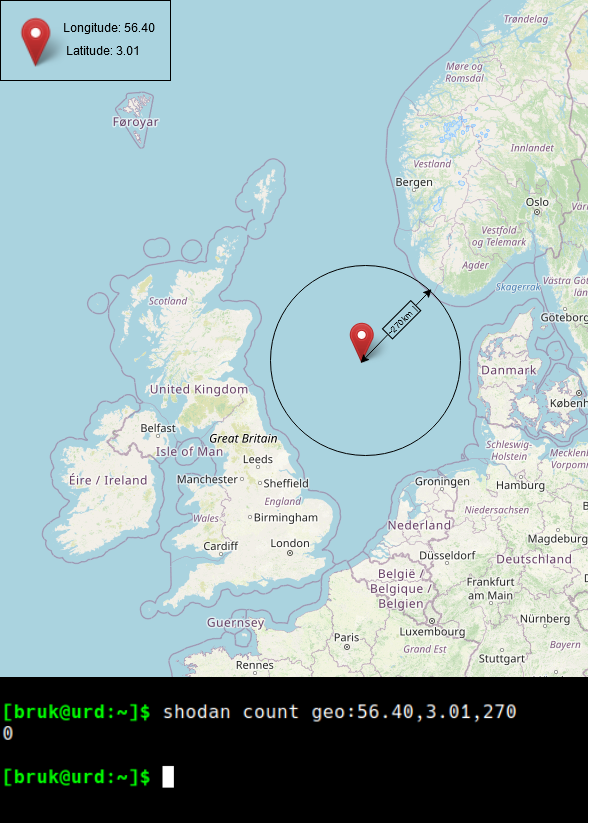
\includegraphics[scale=0.5]{Figurer/geolocation.png}
    \caption{Shodan "geo" filter visualized. Map copyright: https://www.openstreetmap.org/copyright}
    \label{fig:geolocation}
\end{figure}

This query returns zero hits, which shows that the reverse geolocation approach does not work. One possible explanation for this is that the devices are registered in one location, while they are physically located at another. As mentioned in \cref{sec:geo_method}, it is not clear how Shodan find locations, and therefore hard to decide how accurate the information can be.

\subsection{Latency and traceroute} \label{sec:latency_results}
As this project does not have access to any tools that index traceroute latencies, it is not possible to parse trough large quantities of IP address latencies. Therefore, to show how this approach works, the Cobham Seatel Satcom antenna example from \cref{sec:banner_results} will be used, as these devices is already confirmed within the constraints. The traceroute command is simple: "traceroute IP\_ADDRESS". A graph of the latencies from the traceroute can be seen in \cref{fig:traceroute_graph}.

\begin{figure} [H]
    \centering
    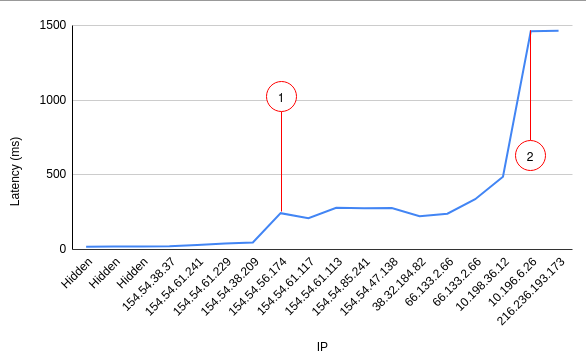
\includegraphics[scale=0.7]{Figurer/latency_graph_marked.png}
    \caption{A visualization of the mean latencies from the traceroute command on the IP address 216.236.193.173.}
    \label{fig:traceroute_graph}
\end{figure}

Two points on this graph is worth mentioning. The first point (1), where the latency has a \~200ms jump, could be a undersea cable.From a Shodan query for the destination IP address, it is found to be in USA, so this is probably when the signal crosses the Atlantic Ocean. The next point on the graph (2), increase the latency by \~1000ms. As the antenna is connected to the internet via satellite, this is probably when the signal travel from land, trough the satellite to the antenna.

With access to large datasets of traceroute latencies, it could be possible to identify devices that have big latency jumps. While this could not prove that a device is located at sea, it would be useful to find subsets of IP addresses that could be investigated further.

\subsection{Combination of methods} \label{sec:combo}
As seen, different methods of identifying devices connected to the internet each have strengths and weaknesses. As the methods use different properties to investigate devices, they can be combined to find devices within the constraints. An example follows.
As mentioned in \cref{sec:banner_results}, the devices identified all used the same port: 161, the standard port for Simple Network Management Protocol (SNMP). \cite{www_ports}. This protocol is used for general purposes, but maybe it is popular for use in usecases like the Cobham antenna found earlier. To test this, a search is made for IP addresses owned by Marlink, which use this port. The search "isp:marlink port:161" returns 2 hits: "193.220.145.36" and "193.220.155.39". The traceroute command is used to check the latencies of these IP addresses.

\begin{figure} [H]
    \centering
    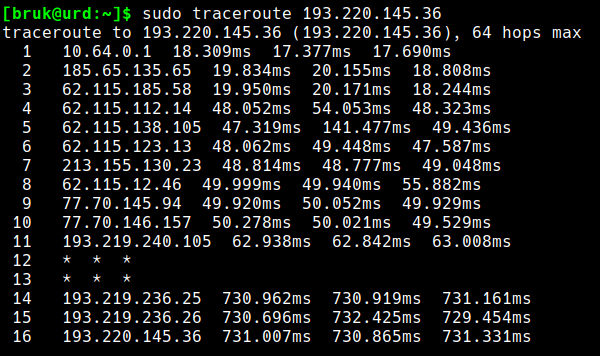
\includegraphics[scale=0.4]{Figurer/marlink_161_2.png}
    \caption{Traceroute command on 193.220.145.36.}
    \label{fig:marlink_traceroute_2}
\end{figure}

\begin{figure} [H]
    \centering
    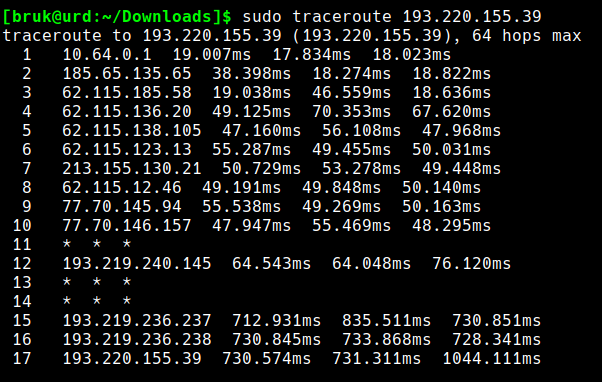
\includegraphics[scale=0.4]{Figurer/marlink_161_1.png}
    \caption{Traceroute command on 193.220.155.39.}
    \label{fig:marlink_traceroute_1}
\end{figure}

Both of these devices show the same jump in latency as the test in \cref{sec:latency_results}, indicating that the device could be connected trough satellite. Due to this device also having a Marlink IP address, the confidence is high that it is present on a ship in the maritime industry. Two of the constraints have been fulfilled: The system is connected to the internet, and is most likely part of the maritime industry. 

Next step is to check for the last constraint: if the system is a Cyber-Physical System(CPS). The "data" field in the banners, as seen in \cref{fig:marlink_traceroute_data}, show that one of the devices is labeled as a "Videoconferencing Device" and the other as a "RouterOS RB750". It should be mentioned that the system administrators owning these devices have the ability to write any label on them, so this could be a lie. This form of security trough obscurity have been advocated, for example in \cite{bodenheim_butts_dunlap_mullins_2014}. With this in mind, the labels are assumed to show the true nature of the devices. 
The videoconferencing device is definitively not part of a CPS. 
A search for the router shows that is is a MicroTik RB750 router, intended for office use.\cite{RB750} This means it is most likely part of a CPS, although this is not definitive. The router could still provide internet to devices in a CPS, making it a part of the CPS. It could also be providing internet access to an employees laptop, where the laptop in turn is connected to a CPS. Either way, there is no way to know for sure without gaining access to the router. Since it is connected to the internet, potential attacker have the ability to try and gain this access.

\begin{figure} [H]
    \centering
    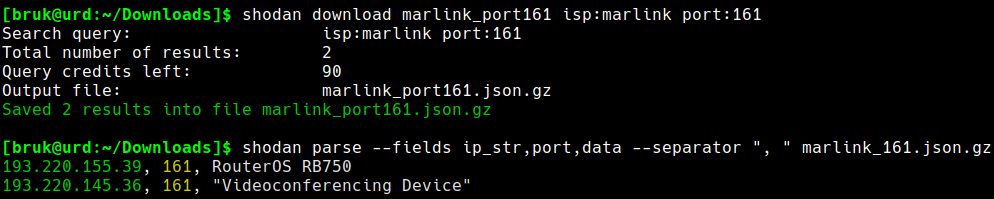
\includegraphics[scale=0.4]{Figurer/marlink_161_data.png}
    \caption{A look at a Shodan search and data from devices found.}
    \label{fig:marlink_traceroute_data}
\end{figure}

\newpage

%

\section{Search Terms Shodan} \label{sec:search_term}
This list is temporary, and more to remember past searches than to actually use in a final report.
\begin{table}[H]
\centering
\begin{tabular}{|l|l|l|}
\hline
Search term & Hits & Found \\ \hline
inmarsat & 7 & From \cite{maritime_pen_test} \\ \hline
Sailor 900 & 3 & From \cite{maritime_pen_test} \\ \hline
Sailor & 32 & From \cite{maritime_pen_test} \\ \hline
thrane & 5 & From \cite{maritime_pen_test} \\ \hline
marlink & 32 &  From thrane search, keywork on one of hits \\ \hline
sealink & 4 &  from marlink website\\ \hline
xchange & 82 &  from marlink website. Possibly name used for different things\\ \hline
navtex & 2 &  from \cite{maritime_digitalization}\\ \hline
nbdp & 3 &  from \cite{maritime_digitalization}\\ \hline
gmdss & 16 &  from \cite{maritime_digitalization}\\ \hline
AIS & 2876 &  from \cite{maritime_digitalization}\\ \hline
furuno & 5 &  from \cite{maritime_digitalization}\\ \hline
LRIT & 12 &  from \cite{maritime_digitalization}\\ \hline
radar & 734 &  a lot of ships have radar right?\\ \hline
MArine Stabilized Antenna System & 23 &  "Hacking Yatch remotely" PowerPoint\\ \hline
E2500 & 774 &  Maretrons nettside\\ \hline
isp:tampnet & 95 &  tampnet is a internet provider for offshore systems\\ \hline
net:185.96.40.0/23 & 23 &  used https://api.hackertarget.com/aslookup/?q=185.96.41.27\\ \hline
net:185.96.40.0/23 & 30 &  same as previous, but using ZoomEye\\ \hline

port:10110 & 4 &  List of TCP and UDP ports, NMEA\\ \hline
NMEA & 67 &  NMEA is a maritime communication protocol\\ \hline


search & hits &  found\\ \hline
\end{tabular}
\end{table}


%%https://en.wikipedia.org/wiki/NMEA_2000_PGN
\Section{Conclusion} \label{sec:conclusion}
The different methods suggested in \cref{sec:method} and tested in \cref{sec:results} were found to have different strengths and weaknesses. To summarize the most important characteristics of each method:

\begin{outline}[itemize]
    \setlength\itemsep{10em}
        \1 Banner Similarities
        \2 Pinpoint an exact device model
        \2 Hard to find identifying device banner
        \1 Internet Service Provider and IP ranges
        \2 Will provide a subset of plausible devices
        \1 Reverse IP geolocation
        \2 Does not work
        \1 Latency and traceroute
        \2 Can be used to give more confidence in identifying a device.

\end{outline}

This shows that the process of identifying devices connected to the internet has many different aspects, and it takes more than one method to be able to identify a device.

Even with these methods, the findings from \cref{sec:results} were either inconclusive or few. Filtering devices on the ISP Marlink proved to find most devices. However, it was difficult to know whether these devices were part of a Cyber-Physical System(CPS) or not. Instead, the list of devices returned would be more useful for performing further research. 

The search for "Maritime Stabilized Antenna System" from \cref{sec:banner_results}, gives few, but decisive identifications of devices. As stated in \cref{sec:intro}, the more devices connected to the internet, the higher potential for vulnerabilities. Therefore, it is good that it is possible to find only a few online devices. These findings should not be seen as conclusive, as only a superficial search was performed. Many devices may still be connected to the internet, even though thet were not found by this project. As mentioned in \cref{sec:further_work}, a more thorough search would include automated scripts for either crawling the internet or parsing datasets. 

Using traceroute to identify devices based on latency is not conclusive, but improves the chance that the right devices are found. This is the only tool that Shodan does not provide, which makes it interesting as a supplement. It should be mentioned that when Shodan queries are sent, they are found in a Shodan database. Shodan has made all the connections to find the devices. With traceroute however, a ping is sent from the device that runs the command. The information is real-time, and the IP address of the sender can be read by the device that receives the traceroute ping. It is not illegal to ping a computer available on the public internet, however, the use of Shodan is more anonymous. 

All in all, the main product of this report is to have defined methods for identifying devices connected to the internet, while the results from testing these methods should be concidered as examples rather than conclusive results. 

\section{Further work} \label{sec:further_work}
When the methods for finding devices connected to the internet, described in \cref{sec:method} was implemented in \cref{sec:results}, the implementations were manual. This was intended to show an example of the method. It should be possible to implement these methods as some kind of crawlers, or parsers for datasets.

Information gathering from the internet is a popular business, and datasets about a lot of different things should be available. For example, as mentioned in \cref{sec:latency_results}, a dataset for traceroute data from all available IP addresses would be useful. 

As mentioned in \cref{sec:limits}, Shodan is not the only alternative for use as crawler. It would be interesting to see if \href{https://censys.io/}{\color{blue}{Censys}}\cite{censys} and \href{www.zoomeye.org}{\color{blue}{ZoomEye}}\cite{zoomeye} would provide different results.

%\section{WORK IN PROGRESS} \label{sec:new}












%% Appendix
\newpage
\begin{appendices} \label{appendix}
\input{"appendix/acronyms"}
%\input{"appendix/project_announcement"}
\section{API commands}
Commands used for interacting with the Shodan API. Both using the Shodan REST APi directly \cite{api_ref} and the Shodan Python Command Line Interface(CLI)\cite{cli_ref}.

\begin{lstlisting}[label=lst:api_ports,caption=Ports web API call]
https://api.shodan.io/shodan/ports/?key={YOUR_API_KEY}
\end{lstlisting}
\input{"appendix/search_filters"}
\input{"appendix/banner_example"}
\end{appendices}


%% References
\newpage
\bibliography{references}{}
\bibliographystyle{plain}



\end{document}
